% ==========================================
% BÖLÜM 1: SORUN GİDERME VE RİSK RAPORU
% ==========================================
\chapter{Sorun Giderme}

Uygulamanın kullanımı sırasında karşılaşılabilecek güvenlik engellemeleri, kütüphane bağımlılıkları ve teknik aksaklıklar ile çözüm adımları aşağıda detaylandırılmıştır.

\vspace{0.4cm}

\begin{itemize}
    \item \textbf{Güvenlik, Makro ve Antivirüs Engellemeleri:}
    \begin{itemize}
        \item \textbf{VBA Makro Engeli:} Kullanıcı dosyayı açtığında makrolar etkinleştirilmezse \texttt{Workbook\_Open} tetiklenmez ve arayüz panelleri yüklenmez. Dosya açıldığında üst barda çıkan \textbf{"İçeriği Etkinleştir"} (\textit{Enable Content}) uyarısı onaylanmalıdır.
        
        \vspace{0.2cm}
        
        \item \textbf{MOTW (Mark of the Web) ve İnternet Engeli:} Dosya ağ üzerinden veya e-posta ile indirildiğinde Windows dosyayı engelleyebilir ve makroların çalışmasını durdurabilir. Dosya sağ tıklanıp Özellikler (\textit{Properties}) penceresinden en alttaki \textbf{"Engellemeyi Kaldır"} (\textit{Unblock}) kutucuğu işaretlenip Kaydet edilmelidir.
    \end{itemize}
\end{itemize}

\vspace{0.2cm}
% --- MOTW GÖRSELİ ---
\begin{figure}[htbp]
    \centering
    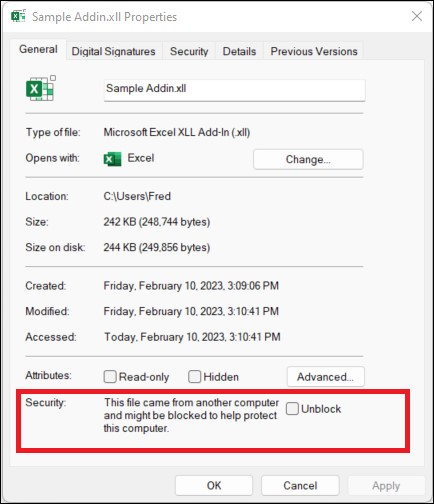
\includegraphics[width=0.35\textwidth]{file-properties-error.jpg}
    \caption{Windows MOTW Güvenlik Engeli ve Unblock (Engellemeyi Kaldır) Seçeneği}
    \label{fig:motw_unblock}
\end{figure}

\begin{itemize}
    \item[] \textbf{ActiveX Denetimleri ve Güvenlik Sınırlamaları:} Kod dinamik olarak \texttt{Forms.Frame.1}, \texttt{Forms.CommandButton.1} gibi OLE nesneleri oluşturur. Office güvenlik güncellemeleri veya Kill-Bit politikaları ActiveX denetimlerinin çalışma anında (\textit{runtime}) eklenmesini engelleyebilir. Excel Trust Center (Güven Merkezi) ayarlarından ActiveX denetimlerinin engellenmediğinden emin olunmalıdır.
\end{itemize}

% ==========================================
% AYRI SAYFA: KÜTÜPHANE VE EKSİK BİLEŞEN HATALARI
% ==========================================
\newpage

\paragraph{Kütüphane ve Eksik Bileşen (Reference) Hataları}
\vspace{0.2cm}

\begin{itemize}
    \item \textbf{Scripting.Dictionary (Windows Bağımlılığı):} Kod içerisinde \texttt{CreateObject \\ ("Scripting.Dictionary")} kullanılmıştır. macOS (Mac için Excel) üzerinde \texttt{scrrun.dll} bulunmadığı için kod \textit{Run-time error 429} hatası verir. Uygulama yalnızca Windows işletim sisteminde çalıştırılmalıdır.
    
    \vspace{0.3cm}
    
    \item \textbf{MSForms (Microsoft Forms 2.0 Object Library) Bağımlılığı:} Panel nesneleri \texttt{MSForms.Frame}, \texttt{MSForms.CommandButton} tipleriyle tanımlanmıştır. Excel kurulumunda VBA desteği eksikse veya nesne kütüphanelerinde bozulma (\textit{MISSING}) varsa "\textit{User-defined type not defined}" hatası alırsınız.
    
    Bu hatayı düzeltmek için klavyeden \textbf{\texttt{Alt + F11}} tuşlarına basarak VBA Editörüne girilmelidir. VBA penceresinde üst menüden \texttt{Tools -> References} seçeneğine tıklanmalı (Bkz. Şekil~\ref{fig:vba_references_all}) ve açılan listede \textit{Microsoft Forms 2.0 Object Library} kutucuğu işaretlenerek onaylanmalıdır.
\end{itemize}

\vspace{0.3cm}

% --- YAN YANA GÖRSELLER ---
\begin{figure}[htbp]
    \centering
    \begin{minipage}{0.45\textwidth}
        \centering
        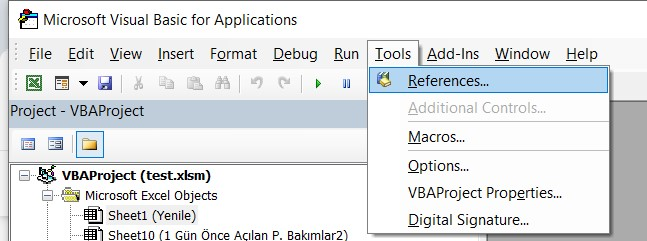
\includegraphics[width=\textwidth]{references1.jpg}
    \end{minipage}
    \hfill
    \begin{minipage}{0.45\textwidth}
        \centering
        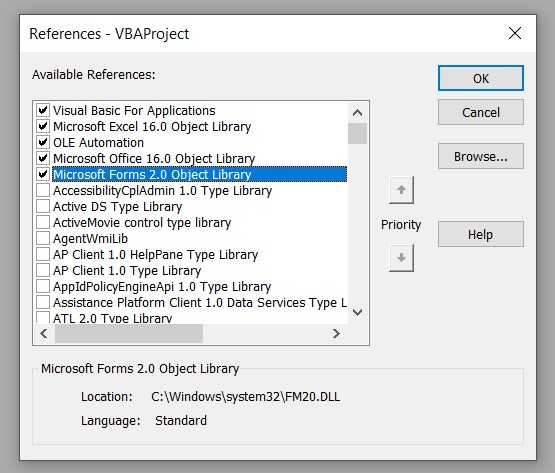
\includegraphics[width=\textwidth]{references2.jpg}
    \end{minipage}
    \caption{Alt + F11 ile VBA Editörüne Erişildikten Sonra Referans Ekleme Adımları (Solda: Tools -> References Menüsü, Sağda: MS Forms 2.0 Seçimi)}
    \label{fig:vba_references_all}
\end{figure}

\vspace{0.3cm}

\begin{itemize}
    \item \textbf{Arayüz Panellerinin Yüklenmemesi ve Manuel Yenileme:} Uygulama açılışında paneller temizlenip otomatik olarak yeniden inşa edildiği için (\texttt{Workbook\_Open} tetiklenmesiyle), ilk açılışta paneller görünmezse en pratik çözüm \textbf{dosyayı kaydedip kapatmak ve tekrar açmaktır}.
    
    Alternatif olarak; dosyayı kapatmadan panelleri yeniden yüklemek isterseniz, \textbf{"Yenile"} çalışma sayfasındayken klavyeden \textbf{\texttt{Alt + F8}} kısayol tuşlarına basabilir, açılan makro penceresinden \texttt{InitializeAppUI} fonksiyonunu seçerek \textbf{"Çalıştır"} (\textit{Run}) butonuna tıklayabilirsiniz.
\end{itemize}